%------------------------------------
\chapter{Thermal Instability}
%------------------------------------
%------------------------------------
\section{Q 2.3: Boussinesq Convection with Rotation - by PA}
%-------------------------------------
The governing equations are given by
\begin{subequations}
 \begin{equation}
  \frac{D\boldsymbol{u}_{i}}{Dt} + 2 (\boldsymbol{\Omega} \times \boldsymbol{u})_{i} = -\nabla \left(\frac{p}{\rho_{0} + gz} + \frac{1}{2}(\boldsymbol{\Omega} \times \boldsymbol{x})_{i}^{2}\right) + g ( 1 - \alpha  (\theta_{0} - \theta) ) \delta_{i3} + \nu \nabla^{2} \boldsymbol{u}_{i}
 \end{equation}
 %
 \begin{equation}
  \frac{\partial \boldsymbol{u}_{j}}{\partial \boldsymbol{x}_{j}} = 0
 \end{equation}
 %
 \begin{equation}
  \frac{D\theta}{Dt} = \kappa \nabla^{2} \theta
 \end{equation}
\end{subequations}

Where $\boldsymbol{u}$ is the velocity in the rotating frame of reference (rotating with the angular velocity $\boldsymbol{\Omega} = \Omega \boldsymbol{\hat{k}}$) and $\theta_{0}$ is the temperature of the bottom layer.

The basic state is given by
\begin{equation}
 \boldsymbol{U} = \boldsymbol{0}, P = - \frac{(\rho_{0} + gz)}{2} (\boldsymbol{\Omega} \times \boldsymbol{x})_{i}^{2}, \Theta = \theta_{0} - \beta z
\end{equation}

where $\beta = (\theta_{0} - \theta_{1})/d$ is the basic temperature gradient. Perturbing about the basic state, we get

\begin{subequations} \label{eq:2_3_perturbed}
 \begin{equation}\label{eq:2_3_perturbed_mom}
  \frac{D\boldsymbol{u}_{i}}{Dt} + 2 (\boldsymbol{\Omega} \times \boldsymbol{u})_{i} = -\nabla \left(\frac{p}{\rho_{0} + gz}\right) + \alpha g (\theta - \theta_{0}) \delta_{i3} + \nu \nabla^{2} \boldsymbol{u}_{i}
 \end{equation}
 %
 \begin{equation}
  \frac{\partial \boldsymbol{u}_{j}}{\partial \boldsymbol{x}_{j}} = 0
 \end{equation}
 %
 \begin{equation}
  \frac{D\theta}{Dt} = \kappa \nabla^{2} \theta
 \end{equation}
\end{subequations}

Where $\boldsymbol{u}, p, \theta$ are now perturbed velocity, pressure and temperature fields. 

It is easy to check that $2\boldsymbol{\Omega \hat{k}} \times \boldsymbol{u} =  (-2\Omega v)\boldsymbol{\hat{i}} + (2\Omega u)\boldsymbol{\hat{j}}$. This immediately implies  $\nabla \times (2\boldsymbol{\Omega \hat{k}} \times \boldsymbol{u}) = \frac{\partial (-2\Omega u)}{\partial z} \boldsymbol{\hat{i}} + \frac{\partial (-2\Omega v)}{\partial z} \boldsymbol{\hat{j}}  + 2\Omega\left(\frac{\partial u}{\partial x} + \frac{\partial v}{\partial y}\right) \boldsymbol{\hat{k}} = = \frac{\partial (2\Omega u)}{\partial z} \boldsymbol{\hat{i}} + \frac{\partial (2\Omega v)}{\partial z} \boldsymbol{\hat{j}}  - 2\Omega\frac{\partial w}{\partial z} \boldsymbol{\hat{k}}$ since $\nabla \cdot \boldsymbol{u} = 0$. Therefore, $\nabla \times (2\boldsymbol{\Omega \hat{k}} \times \boldsymbol{u}) = -2\Omega \frac{\partial \boldsymbol{u}}{\partial z}$. Now, considering only linear terms in perturbation quantities, for example,
$\frac{D\theta}{Dt} = \frac{\partial \theta}{\partial t} - \beta w$, etc. and taking the curl of Eqn. (\ref{eq:2_3_perturbed_mom}), we get the perturbation vorticity equation and the perturbation temperature equation:
\begin{subequations}
 \begin{equation}\label{eq:2_3_perturbed_vorticity}
\frac{\partial \boldsymbol{\omega}}{\partial t} - 2\Omega\frac{\partial \boldsymbol{u}}{\partial {z}} = \alpha g \nabla \theta \times \boldsymbol{\hat{k}} + \nu \nabla^{2} \boldsymbol{\omega}.  
 \end{equation}
 %
 \begin{equation} \label{eq:2_3_perturbed_energy}
  \frac{\partial \theta}{\partial t} - \beta w = \kappa \nabla^{2} \theta
 \end{equation}
\end{subequations}

In particular taking the third component of the perturbation vorticity equation \ref{eq:2_3_perturbed_vorticity}, we obtain

\begin{equation}\label{eq:2_3_perturbed_vorticity_z}
 \frac{\partial \omega_{3}}{\partial t} - 2\Omega\frac{\partial w}{\partial {z}} = \nu \nabla^{2} \omega_{3}.
\end{equation}

Taking the curl of the perturbation vorticity equation again, we obtain
\begin{align}\label{eq:2_3_curl_perturbed_vorticity}
\begin{split}
 -\frac{\partial \nabla^{2}\boldsymbol{u}}{\partial t} - 2\Omega \frac{\partial \boldsymbol{\omega}}{\partial {z}} &= \alpha g \left(\nabla\left(\frac{\partial \theta}{\partial z} - \nabla^{2} \theta\boldsymbol{\hat{k}}\right) \right) - \nu \nabla^{4} \boldsymbol{u}\\
\textrm{taking the third component} &  \Rightarrow  \\
\left(\frac{\partial}{\partial t} - \nu \nabla^{2}\right) \nabla^{2} w &= \alpha g \Delta_{1} \theta - 2 \Omega \frac{\partial \omega_{3}}{\partial z},
\end{split}
\end{align}

where $\Delta_{1} = \frac{\partial^{2}}{\partial x^{2}} + \frac{\partial^{2}}{\partial y^{2}}$ is the horizontal Laplacian.

Hence we obtain the system of linearized equations in the perturbation quantities
\begin{subequations}\label{eq:2_3_perturbed_linear}
\begin{equation}
 \left(\frac{\partial }{\partial t} - \kappa \Delta \right) \theta = \beta w
 \end{equation}
 \begin{equation}
  \left(\frac{\partial }{\partial t} - \nu \Delta \right) \omega_{3} = 2\Omega\frac{\partial w}{\partial {z}}
 \end{equation}
  \begin{equation}
\left(\frac{\partial }{\partial t} - \nu \Delta \right) \Delta w = \alpha g \Delta_{1} \theta - 2 \Omega \frac{\partial \omega_{3}}{\partial z}
\end{equation}
\end{subequations}

The normal mode ansatz is

$(w, \theta, \omega_{3}) = (W, T, Z)f e^{st}, \Delta_{1} f + a^{2}f = 0$, where $a^{2}$ is an arbitrary constant arising from separation of variables (see text). Substituting the normal mode ansatz into Eqns.(\ref{eq:2_3_perturbed_linear}), we obtain

\begin{subequations}\label{eq:2_3_amplitude}
 \begin{equation}
  (D^{2}-a^{2}-s)Z = -\mathcal{T}^{1/2}DW
 \end{equation}
 
 \begin{equation}
  (D^{2}-a^{2}-s) T = -W
 \end{equation}
 
 \begin{equation}
  (D^{2}-a^{2})(D^{2}-a^{2}-s/Pr)W = a^{2}RT - \mathcal{T}^{1/2}DZ
 \end{equation}
\end{subequations}
where $\mathcal{T} = 4\Omega^{2}d^{4}/\nu^{2}$ is the Taylor number and $D = d/dz$.

Eliminating $T$ and $Z$, we obtain a single equation for $W$.

\begin{equation}\label{eq:rotating_RB_W_eqn}
 (D^{2}-a^{2}-s)\left( (D^{2}-a^{2}-s/Pr)^{2}(D^{2}-a^{2}) + \mathcal{T}D^{2}\right)W = -a^{2}R (D^{2}-a^{2}-s/Pr)W
\end{equation}

%-------------------------------------
%-------------------------------------
\section{Q 2.7: Analytical Solution for Rigid-Rigid Boundaries - by PA}
%-------------------------------------
The marginal states (corresponding to $s=0$, where $s$ is the eigenvalue) are given by Eqn.($10.9$) subject to boundary conditions given in Eqn. ($10.10$). We rewrite them here as Eqn.(\ref{eq:2_7_rb_marginal}), Eqn.(\ref{eq:2_7_rb_rigid_rigid_bc}) for the sake of completeness 

\begin{equation}\label{eq:2_7_rb_marginal}
 (D^{2}-a^{2})^{3} W = - a^{2} R W
\end{equation}
\begin{equation}\label{eq:2_7_rb_rigid_rigid_bc}
 W = DW = (D^{2}-a^{2})^{2} W = 0 \textrm{ at } z = 0, 1
\end{equation}

where $D = d/dz$ and $a$ is the arbitrary constant (obtained from the separation of variables, to be determined as a part of the problem). 

To solve Eqn.(\ref{eq:2_7_rb_marginal}), we substitute 

\begin{equation}\label{eq:2_7_W_ansatz}
W = e^{q(z-1/2)}  
\end{equation}

This gives

\begin{equation}\label{eq:2_7_rb_marginal_roots}
 (q^{2}-a^{2})^{3} = - a^{2} R = -a^{6} \tau^{3}.
\end{equation}

Peeking at the solution at the back of the book, we further substituted $R = a^{4}\tau^{3}$, where $\tau = \mathcal{T}^{1/2}$, the square root of the Taylor number $\mathcal{T} = 4\Omega^{2}d^{4}/\nu^{2}$. 

Therefore, 

\begin{equation}
 q^{2}-a^{2} = -a^{2}\tau \times (1 \textrm{, } \omega \textrm{ or } \omega^{2}),
\end{equation}

with $\omega = \exp{(2\pi i/3)}$ being the cube root of unity.

$\Rightarrow$
$$q = a (1- \tau \times (1 \textrm{, } \omega \textrm{ or } \omega^{2}))^{1/2} $$

Therefore
\begin{equation}\label{eq:2_7_q_roots}
 q = iq_{0}, q_{1}, q_{2} ( =  q^{*}_{1})
\end{equation}
with $q_{0} = a (\tau - 1)^{1/2}, q_{1} = a (1 - \tau \omega)^{1/2}, q_{2} = a (1 - \tau \omega^{2})^{1/2} = q^{*}_{1}$. 

From Eqn. (\ref{eq:2_7_W_ansatz}) and Eqn. (\ref{eq:2_7_q_roots}), the even solution (about $z = 1/2$) can now be written as

\begin{equation}\label{eq:2_7_even_soln}
\boxed{
 W = A_{0} \cos{[q_{0}(z-1/2)]} + A_{1} \cosh{[q_{1}(z-1/2)]} + A^{*}_{1} \cosh{[q^{*}_{1}(z-1/2)]}
 }.
\end{equation}

Now, let us apply boundary conditions Eqn. \ref{eq:2_7_rb_rigid_rigid_bc}. Since we are considering an even solution and the problem is symmetric with respect to the boundaries, we will only apply them at $z= 0$.  

\begin{align}\label{eq:2_7_apply_bc_naive}
 \begin{split}
  A_{0} \cos{(q_{0}/2)} + A_{1}\cosh{(q_{1}/2)} + A^{*}_{1}\cosh{(q^{*}_{1}/2)} & = 0 \\
  %
  -A_{0}q_{0}\sin{(q_{0}/2)} + A_{1}q_{1}\sinh{(q_{1}/2)} + A^{*}_{1}q^{*}_{1}\sinh{(q^{*}_{1}/2)} & = 0\\
  %
  A_{0}(q_{0}^{2} + a^{2})^{2}\cos{(q_{0}/2)} + A_{1}(q_{1}^{2} - a^{2})^{2}\cosh{(q_{1}/2)} + A^{*}_{1}({q^{*}_{1}}^{2} - a^{2})^{2}\cosh{(q^{*}_{1}/2)}  & = 0 \\
  %
  \textrm{i. e.}\\
  A_{0}\cos{(q_{0}/2)} + A_{1}\omega \cosh{(q_{1}/2)} + A^{*}_{1}\omega \cosh{(q^{*}_{1}/2)} & = 0.
 \end{split}
\end{align}

Substituting $A_{0} \cos{(q_{0}/2)} = A'_{0}, A_{1}\cosh{(q_{1}/2)} = A'_{1}$ and $A^{*}_{1}\cosh{(q^{*}_{1}/2)} = A'^{*}_{1}$
%
\begin{equation}\label{eq:2_7_matrix_form}
\begin{bmatrix}
1   &   1   &   1 \\
\tan({q_{0}/2})   &   \tanh({q_{1}/2})   &   \tanh({q^{*}_{1}/2})\\
1   &   \omega &   \omega^{*}\\
\end{bmatrix}
\begin{bmatrix}
 A'_{0}\\
 A'_{1}\\
 A'^{*}_{1}\\
\end{bmatrix} 
= \boldsymbol{0}.
\end{equation}

For Eqn. (\ref{eq:2_7_matrix_form}) to have nontrivial solutions, the determinant of the matrix must be zero. This gives the required eigenvalue relation

\begin{equation}\label{eq:2_7_rigid_rigid_eig}
\boxed{
 Im \{(\sqrt{3} + i)q_{1} \tanh{(q_{1}/2)} \} + q_{0} \tan{(q_{0}/2)} = 0
 }.
\end{equation}

To find the critical Rayleigh number $R_{c}$ and corresponding $a_{c}$, we have to solve Eqn. \ref{eq:2_7_rigid_rigid_eig} recursively. From \cite{reid1958some}, we obtain $a_{c} = 3.117, R_{c} = 1707.762$. 
%-------------------------------------
\subsection{Bonus: Odd solution}
Proceeding as above, we can also write the odd solution (about $z = 1/2$) as follows

\begin{equation}\label{eq:2_7_odd_soln}
\boxed{
 W = A_{0} \sin{[q_{0}(z-1/2)]} + A_{1} \sinh{[q_{1}(z-1/2)]} + A^{*}_{1} \sinh{[q^{*}_{1}(z-1/2)]}
 }.
\end{equation}

and obtain the counterpart eigenvalue relation Eqn. (\ref{eq:2_7_rigid_rigid_eig}) as


\begin{equation}\label{eq:2_7_rigid_rigid_eig_2}
\boxed{
 Im \{(\sqrt{3} + i)q_{1} \coth{(q_{1}/2)} \} + q_{0} \cot{(q_{0}/2)} = 0
 }.
\end{equation}
%------------------------------------
%------------------------------------
\section{Q 2.10: Instability with Rotation - by PA}
%------------------------------------
A solution to Eqn. (\ref{eq:rotating_RB_W_eqn}) is $W = \sin{j \pi z}$. Substituting in Eqn. (\ref{eq:rotating_RB_W_eqn}), 

\begin{equation}\label{eq:2_10_s_eqn}
 (s + a^{2} + j^{2}\pi^{2})\left( (j^{2}\pi^{2} + a^{2} + s/Pr)^{2}(j^{2}\pi^{2} + a^{2}) + \mathcal{T}j^{2}\pi^{2}\right) = a^{2}R(j^{2}\pi^{2} + a^{2} + s/Pr). 
\end{equation}
Hence, 
\begin{equation}
 R = \frac{(s + a^{2} + j^{2}\pi^{2})\left( (j^{2}\pi^{2} + a^{2} + s/Pr)^{2}(j^{2}\pi^{2} + a^{2}) + \mathcal{T}j^{2}\pi^{2}\right)}{a^{2} (j^{2}\pi^{2} + a^{2} + s/Pr)}
\end{equation}

We will follow the analysis in $\S 29$ of \cite{chandrasekhar1961hydrodynamic}. We note that $s$ can be complex. In order to look for solutions which are oscillatory at the onset, we look for $s$ purely imaginary. Following \cite{chandrasekhar1961hydrodynamic}, \cite{drazin2004hydrodynamic}, we do the following substitutions for the sake of simplicity. 

\begin{equation}\label{eq:2_10_substitutions}
 R = j^{4}\pi^{4}R_{1}, s = i \omega j^{2}\pi^{2} Pr, \mathcal{T} = j^{4}\pi^{4}T_{1}, j^{2}\pi^{2} + a^{2} = j^{2}\pi^{2} y.
\end{equation}

Eqn. (\ref{eq:2_10_s_eqn}) becomes
\begin{equation*}
 j^{2}\pi^{2}(y + i\omega Pr)\left(j^{4}\pi^{4}(y + i\omega)^{2} \cdot j^{2}\pi^{2}y + j^{6}\pi^{4}T_{1}\right) = j^{2}\pi^{2} (y-1)j^{4}\pi^{4}R_{1}\cdot j^{2}\pi^{2}(y + i\omega) 
\end{equation*}

i.e.,
\begin{align}\label{eq:2_10_R1}
 \begin{split}
  R_{1} &= (y + i\omega Pr)\left[y(y + i\omega)^{2} + T_{1} \right]/(y-1)(y+i\omega) \\
  & = (y + i\omega Pr)\left[y(y + i\omega)(y^{2}+\omega^{2}) + T_{1}(y-i\omega)\right]/(y-1)(y^{2}+\omega^{2})
 \end{split}
\end{align}

Since we are looking for $s$ purely imaginary, we assume $\omega$ to be purely real. In general, as argued in $\S 29$ of \cite{chandrasekhar1961hydrodynamic}, Eqn.(\ref{eq:2_10_R1}) would yield a complex $R_{1}$. However, physically, $R_{1}$ is just a scaled Rayleigh number and should be purely real. Hence, we separate out the real and imaginary parts of Eqn.(\ref{eq:2_10_R1}) to obtain
\begin{align}\label{eq:2_10_R1_re_im}
 \begin{split}
  R_{1} &= \left[y(y^{2} + \omega^{2}Pr) (y^{2}+\omega^{2}) + T_{1}(y^{2} + \omega^{2}Pr)\right]/(y-1)(y^{2}+\omega^{2})\\
  0 &= \omega y \left[y(1 + Pr)(y^{2}+\omega^{2}) + T_{1}(Pr - 1) \right]/(y-1)(y^{2}+\omega^{2})
 \end{split}
\end{align}

This implies
\begin{align}\label{eq:2_10_omega_R1_expressions}
 \begin{split}
  \omega^{2} &= T_{1}(1-Pr)/y(1+Pr) - y^{2}\\
  R_{1} &= 2(1+Pr) \frac{\left[y^{3} + \frac{Pr^{2}T_{1}}{(1+Pr)^{2}} \right]}{(y+1)}
 \end{split}
\end{align}

For overstable oscillations, we want $\omega^{2}$ to be real and non-zero, giving, 

\begin{equation}\label{eq:2_10_overstability_cond}
 \boxed{
 T_{1} > y^{3} (1+Pr)/(1-Pr)
 }
\end{equation}
%------------------------------------
%-------------------------------------
\section{Q 2.11: Annular Cells - by PA}
%-------------------------------------
$\Delta_{1} f + a^{2}f = 0$ where $\Delta_{1} = \frac{\partial^{2}}{\partial x^{2}} + \frac{\partial^{2}}{\partial y^{2}}$ is the horizontal Laplacian, takes the form 

\begin{equation}\label{eq:2_11_bessel}
 \frac{d^{2}f}{dr^{2}} + \frac{1}{r}\frac{df}{dr} + a^{2}f = 0
\end{equation}
if $f \equiv f(r)$. The solutions to Eqn. (\ref{eq:2_11_bessel}) are the well-known Bessel functions $f = J_{0}(ar), Y_{0}(ar)$. We discard the $Y_{0}(ar)$ solution because we want f to be bounded as $r \rightarrow 0$. 

Hence,
\begin{align}
 \begin{split}
  f &= AJ_{0}(ar)\\
  w &= A J_{0}(ar) \sin{j\pi z}
 \end{split}
\end{align}

 \begin{figure}[H]
    \centering
    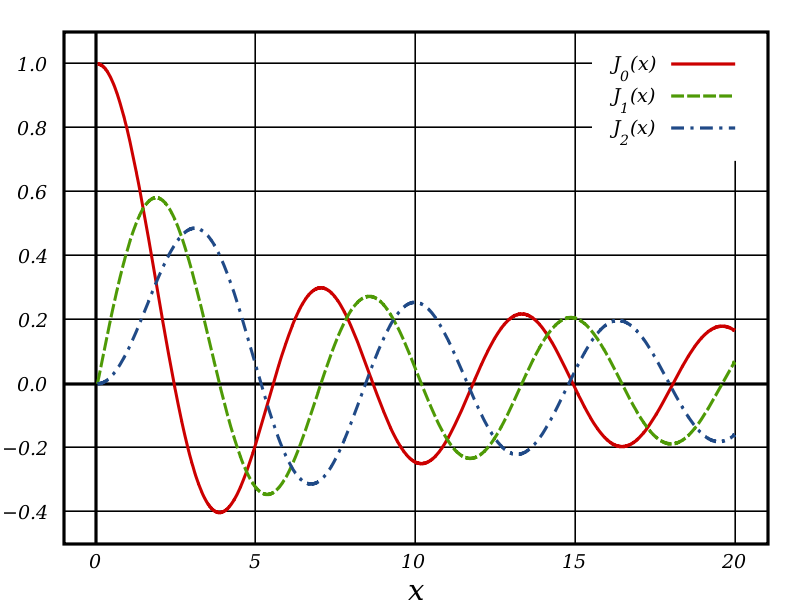
\includegraphics[scale = 0.5]{Figs/Bessel_Functions.png}
    \caption{Bessel functions of the first kind}
    \label{fig:Bessel_Functions}
\end{figure}

Since $J_{0}(ar)$ oscillates from positive to negative and back to positive values, concentric annular cells can exist. 
